% Chapter Template

\chapter{Reflection of your own roles in the team} % Main chapter title

In the team I had the role of core developer. Given my previous experience in developing I think that this was the best role for me in this team. I have almost 4y experience as a full stack developer so i did the web application tweetsAnalytics:\\ \href{https://github.com/lupu60/tweetsAnalytics}{https://github.com/lupu60/tweetsAnalytics}

\begin{figure}[h]
	\centering
	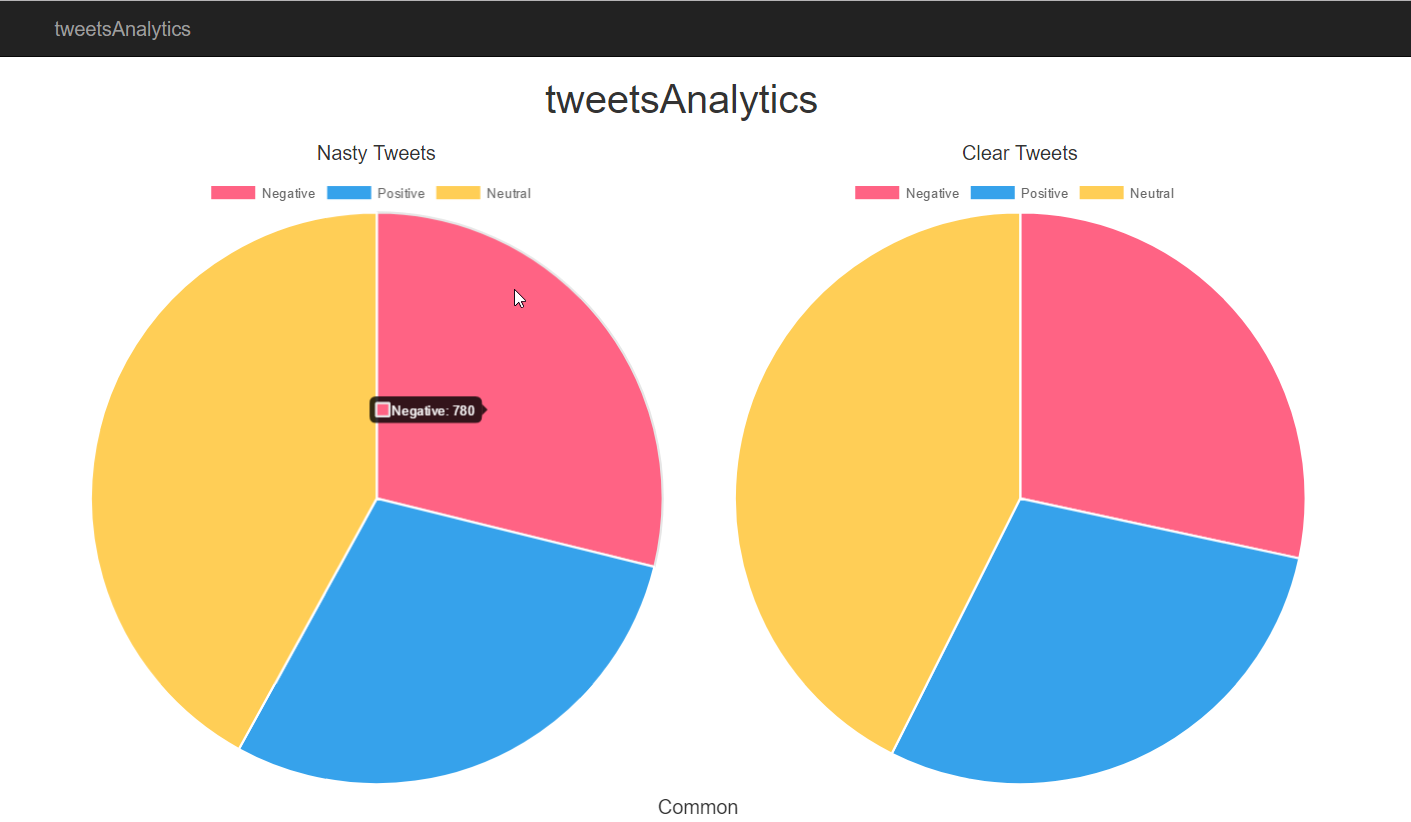
\includegraphics[width=\textwidth]{images/app1.png}
\end{figure}
The core app is written in javascript for frontend and also backend using the javascript framework Expressjs. Node.js is an open source, cross-platform runtime environment for server-side and networking applications. Node.js applications are written in JavaScript, and can be run within the Node.js runtime on OS X, Microsoft Windows, Linux, FreeBSD, NonStop and IBM i.
Node.js provides an event-driven architecture and a non-blocking I/O API that optimizes an application's throughput and scalability. These technologies are commonly used for real-time web applications.
Node.js uses the Google V8 JavaScript engine to execute code, and a large percentage of the basic modules are written in JavaScript. Node.js contains a built-in library to allow applications to act as a Web server without software such as Apache HTTP Server or IIS.
\begin{figure}[h]
	\centering
	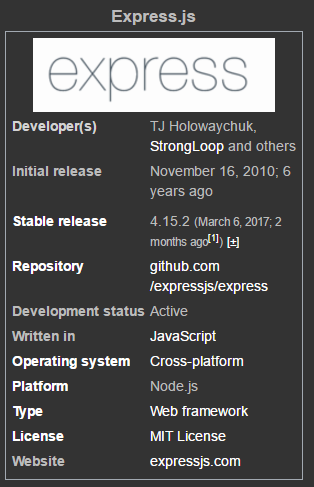
\includegraphics[width=0.5\textwidth]{images/expressjs.png}
\end{figure}
My app is consuming the rest api of the sentiment.vivekn.com and is drowning all the charts with the lib chart.js. The Sentiment analysis (sometimes known as opinion mining or emotion AI) refers to the use of natural language processing, text analysis, computational linguistics, and biometrics to systematically identify, extract, quantify, and study affective states and subjective information. Sentiment analysis is widely applied to voice of the customer materials such as reviews and survey responses, online and social media, and healthcare materials for applications that range from marketing to customer service to clinical medicine.
Generally speaking, sentiment analysis aims to determine the attitude of a speaker, writer, or other subject with respect to some topic or the overall contextual polarity or emotional reaction to a document, interaction, or event. The attitude may be a judgment or evaluation (see appraisal theory), affective state (that is to say, the emotional state of the author or speaker), or the intended emotional communication (that is to say, the emotional effect intended by the author or interlocutor).
\begin{figure}[h]
	\caption{Nodejs logo}
	\centering
	
\includegraphics[width=0.5\textwidth]{images/nodejs-logo.png}
\end{figure}

\begin{figure}[h]
	\centering
	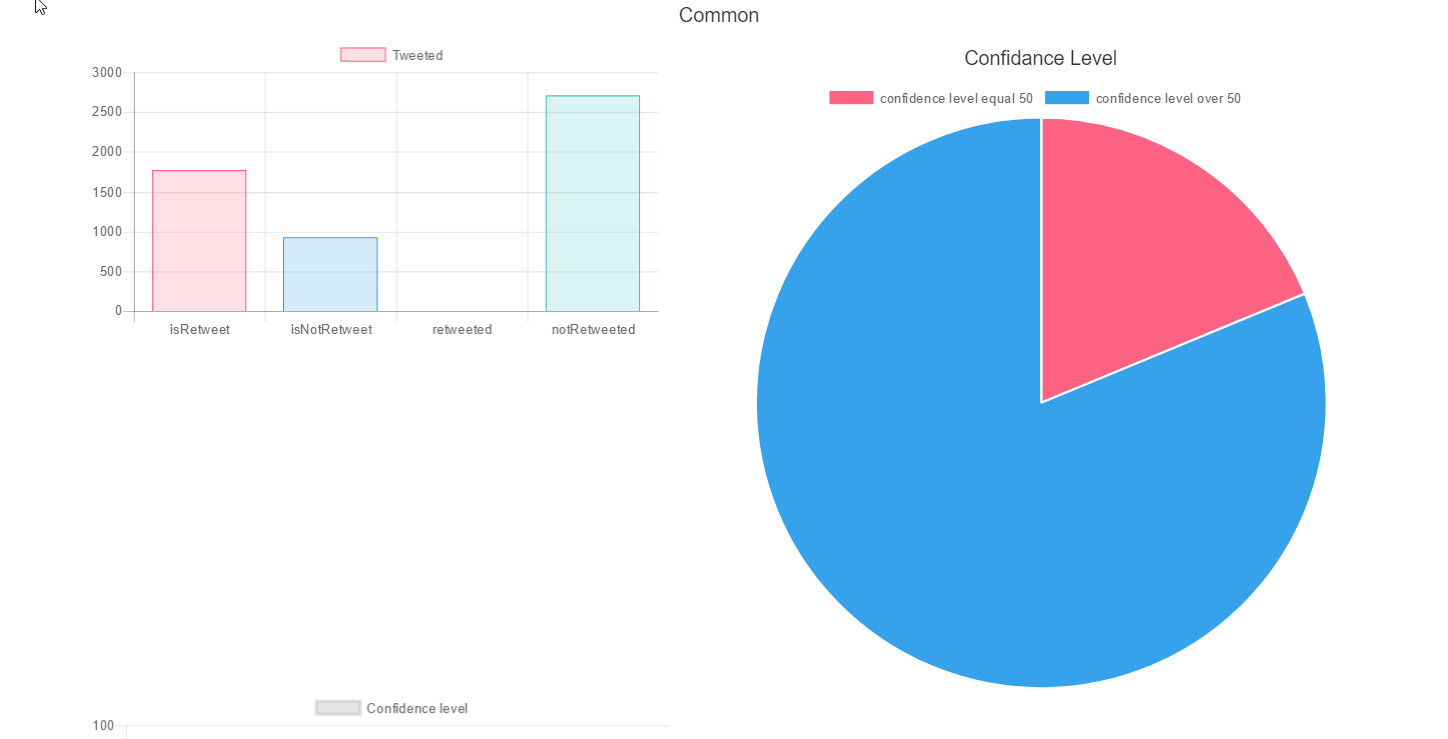
\includegraphics[width=\textwidth]{images/app2.png}
\end{figure}

\vfill

\begin{lstlisting}[language=JavaScript]
var twitterAnalysis = {
    postToSentiment(twietsJson) {
        var sentimentJson = [];
        twietsJson.tweets.forEach(function(element, index) {
            let twiet = {
                "text": element.text,
                "created": element.created,
                "retweetCount": element.retweetCount,
                "isRetweet": element.isRetweet,
                "retweeted": element.retweeted
            }
            var form = new FormData();
            form.append("txt", element.text);
            var settings = {
                "async": false,
                "crossDomain": true,
                "url": "http://sentiment.vivekn.com/api/text/",
                "method": "POST",
                "processData": false,
                "contentType": false,
                "mimeType": "multipart/form-data",
                "data": form
            }

            $.ajax(settings).done(function(response) {
                twiet.confidence = JSON.parse(response).result.confidence
                twiet.sentiment = JSON.parse(response).result.sentiment
                sentimentJson.push(twiet);
                console.log("done");
            });
        });
        this.downloadFile(JSON.stringify(sentimentJson), "sentiment.json");
    }
}
\end{lstlisting}
